\documentclass[a4paper, 12pt]{report}
\usepackage[T1]{fontenc}
\usepackage[utf8]{inputenc}
\usepackage[english]{babel}
\usepackage{mathtools}
\usepackage{amsfonts}
\usepackage{amsmath}
\usepackage{mathrsfs}
\usepackage{enumitem}
\usepackage{booktabs}
\usepackage{array}

% Avoid paragraph indent
\setlength{\parindent}{0pt}
% Useful floor and ceiling functions
\DeclarePairedDelimiter{\floor}{\lfloor}{\rfloor}
\DeclarePairedDelimiter{\ceil}{\lceil}{\rceil}
% Argmax/Argmin notation
\DeclareMathOperator*{\argmax}{argmax} 
\DeclareMathOperator*{\argmin}{argmin} 
% Modified margins
\usepackage[margin=2cm]{geometry}
% This avoids hypenation
\hyphenpenalty=10000
\usepackage{tikz}
\usetikzlibrary{arrows,calc,positioning,shadows,shapes}
\usepackage{graphicx}
\usepackage{subfig}
\graphicspath{{./images/}}
\captionsetup[figure]{labelfont={bf},name={Figure},labelsep=period}
\captionsetup[table]{labelfont={bf},name={Table},labelsep=period}

\usepackage{float}

\begin{document}
	
\title{Digital Communications and Laboratory \\ Fourth Homework}
\author{Faccin Dario, Santi Giovanni}
\date{}
\maketitle

\section*{Transmission system}
In the following, two different scenarios are developed: a single carrier transmission using Receiver (b) of homework 3 and an OFDM transmission with $\mathcal{M}$=512 sub-channels. Both implementations are firstly simulated using coding to improve the error correction capability of the system; in particular, a \textit{Low-density parity check} LDPC encoding is applied to the initial data stream in order to allow the receiver to detect codewords which do not belong to the code $\mathcal{C}$ and eventually to correct them with the use of an LDPC decoder. These functions are provided by the Matlab toolbox. Finally, the same transmission is simulated without coding to appreciate the difference in terms of $P_{bit}$ for varying SNR. \\
In this report we decided to treat only the implementation of the encoded transmission; the uncoded one, indeed, follows by simply removing the LDPC and the interleaver.

\subsection*{Symbols generation}
A data stream of bits $b_l$ is generated using a PN sequence of length $2^{20}-1$ repeated once. This is encoded by an LDPC encoder provided by the Matlab toolbox, which reads sequences of 32400 bits and generates codewords $c_m$ of length 64800 bits. An interleaver is used in order to reduce the probability of having \textit{burst} errors, then a bitmap maps pairs of bits into a QPSK constellation with \textit{Gray coding}. This scenario is given in Figure [\ref{}].

\begin{figure}[H]
	\centering
	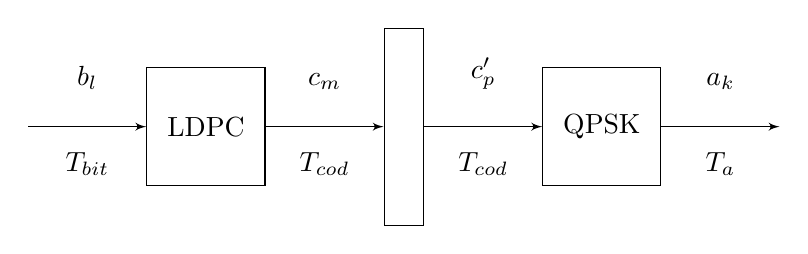
\begin{tikzpicture}[auto,>=latex']
	\tikzstyle{block} = [draw, rectangle, minimum height=1cm, minimum width=1cm]
	
	\node [coordinate] (start) {};
	
	\node [draw, rectangle, minimum height=1.5cm, minimum width=1.5cm, right = 1.5cm of start] (encoder) {LDPC};
	
	\node [draw, rectangle, minimum height=2.5cm, minimum width=0.5cm, right = 1.5cm of encoder] (interl) {};
	
	\node [draw, rectangle, minimum height=1.5cm, minimum width=1.5cm, right = 1.5cm of interl] (qpsk) {QPSK};
	
	\node [coordinate, right = 1.5cm of qpsk] (end) {};
	
	\draw [->] (start) --node[label={[label distance=0.2cm]270:$T_{bit}$}, label={[label distance=0.1cm]90:$b_l$}]{} (encoder);
	
	\draw [->] (encoder) --node[label={[label distance=0.2cm]270:$T_{cod}$}, label={[label distance=0.1cm]90:$c_m$}]{} (interl);
	
	\draw [->] (interl) --node[label={[label distance=0.2cm]270:$T_{cod}$}, label={[label distance=0.1cm]90:$c'_p$}]{} (qpsk);
	
	\draw [->] (qpsk) --node[label={[label distance=0.2cm]270:$T_a$}, label={[label distance=0.1cm]90:$a_k$}]{} (end);
	
	\end{tikzpicture}
\end{figure}

\subsection*{Single Carrier}
The channel for the single carrier transmission is that implemented in homework 3. \\
The receiver filter consists of a filter $g_M$ matched to the transmission filter $q_c$ followed by a \textit{Decision Feedback Equalizer} (DFE) filter. The matched filter is simply computed as $g_m(t) = q^*_c(t_0-t)$, where $t_0$ is the timing phase. Since the global impulse response of the system $h = g_c * g_M$ at the input of  $c$ is defined @$\frac{T}{4}$, a downsampling of a factor 4 is required between the output of $h$ and the input of $c$. The equations used to compute both filters $c$ and $b$ have already been discussed in homework 3. The scenario just described is given in Figure [\ref{Model_SC}].

\begin{figure}[H]
	\centering
	\begin{tikzpicture}[auto,>=latex']
	\tikzstyle{block} = [draw, rectangle, minimum height=1cm, minimum width=1cm]
	
	\node [coordinate, label={[label distance=0.65cm]60:$a_k$}] (start) {};
	\node [block, right = 1.25cm of start] (intpl){$\uparrow 4$};
	\node [coordinate, label={[label distance=0.5cm]90:$a'_n$}, right = 0.75 cm of intpl] (c1) {};
	\node [block, right = 1.25cm of intpl] (imp){$q_c$};
	\node [draw, circle,minimum size=0.5cm,inner sep=0pt, right = 1.25cm of imp] (sum1){$+$};
	\node [coordinate, label={[label distance=0.4cm]90:$s_c(n \frac{T}{4})$}, right = 0.75cm of imp] (c2) {};
	
	\node [coordinate, label={[label distance=0.2cm]90:$w_c(n \frac{T}{4})$}, above = 1cm of sum1] (wgn) {};

	\node [block, right = 1.25cm of sum1] (matchedf){$g_M$};
	\node [coordinate, right = 0.75 cm of matchedf] (c0) {};
	\node [coordinate, above = 0.5 cm of c0, label={[label distance=0.1cm]45:$t_0 + kT$} ] (c1) {};
	
	\node [coordinate, right = 1.2cm of matchedf] (c2) {};
	\node [block, right = 1cm of c2] (cfilter){$c$};
	\node [draw, circle,minimum size=0.5cm,inner sep=0pt, right = 1cm of cfilter] (sum){$+$};
	\node [coordinate, below = 1cm of sum] (c3) {};	
	\node [block, right = 0.5cm of sum] (detector){$\amalg$};
	\node [coordinate, right = 0.5cm of detector] (cfin) {};
	\node [coordinate, below = 1.254cm of cfin] (c6) {};
	\node [block, right = 0.75cm of c3] (b){$b$};	
	\node [coordinate, right = 1cm of detector, label={[label distance=0.1cm]0:$\hat{a}_{k-D}$}] (end){};
	
	\draw [->] (start) --node[label={[label distance=0.2cm]270:$T$}]{} (intpl);
	\draw [->] (intpl) --node[label={[label distance=0.2cm]270:$\frac{T}{4}$}]{} (imp);
	\draw [->] (imp) --node[label={[label distance=0.2cm]270:$\frac{T}{4}$}]{} (sum1);
	\draw [->] (wgn) --node[]{} (sum1);
	\draw [->] (sum1) --node[label={[label distance=0.1cm]90:$r_c(n \frac{T}{4})$}]{} (matchedf);
	\draw [-] (matchedf) --node[label={[label distance=0.2cm]270:$\frac{T}{4}$}]{} (c0);
	\draw [-] (c1) --node[]{} (c2);
	\draw [->] (c2) --node[label={[label distance=0.2cm]270:$T$}]{} (cfilter);
	\draw [->] (cfilter) --node[label={[label distance=0.2cm]270:$T$}]{} (sum);
	\draw [->] (c3) --node[]{} (sum);
	\draw [-] (b) --node[]{} (c3);
	\draw [-] (c6) --node[]{} (b);
	\draw [-] (cfin) --node[label={[label distance=0.1cm]0:$T$}]{} (c6);
	\draw [->] (sum) --node[]{} (detector);
	\draw [->] (detector) --node[]{} (end);
	
	\end{tikzpicture}
	\caption{Model for the SC channel.}
	\label{Model_SC} 
\end{figure}

\clearpage
\subsection*{OFDM}
Orthogonal frequency division multiplexing is an efficient modulation technique by which blocks of $\mathcal{M}$ symbols are transmitted in parallel over $\mathcal{M}$ sub-channels, using $\mathcal{M}$ modulation filters with frequency responses $\mathcal{H}_i(f)$, $i=1,2,\dots,\mathcal{M}-1$. The $\mathcal{M}$ input symbols at the $k_{th}$ modulation interval are represented by the vector

\begin{equation}
\mathbf{a}_k = [a_k[0],\dots,a_k[\mathcal{M}-1]]^T
\end{equation}

where $a_k[i]\in\mathcal{A}[i]$, $i=0,\dots,\mathcal{M}-1$.\\
We implemented the \textit{Discrete Multitone} DMT version in which the transmit and receiver filter backs use a prototipe filter with impulse response given by

\begin{equation}
h_n = \begin{cases}
		1 \quad\quad \text{if } 0\le n\le\mathcal{M}-1 \\
		0 \quad\quad \text{otherwise}
\end{cases}
\end{equation}

In this way the impulse response of the polyphase components of the prototype filter are simply $\{ h_n^{(l)}\}=\{\delta_n\}$ for $l=0,1,\dots,\mathcal{M}$. As a consequence, because the frequency responses are constants, we obtain directly the transmit signal by applying a P/S conversion at the output of the IDFT. To equalise the channel, we implemented the baseband equivalent system given in Figure [\ref{ofdm}]. The channel is given in Figure [\ref{Model_OFDM}]
.
\begin{figure}[H]
	\centering
	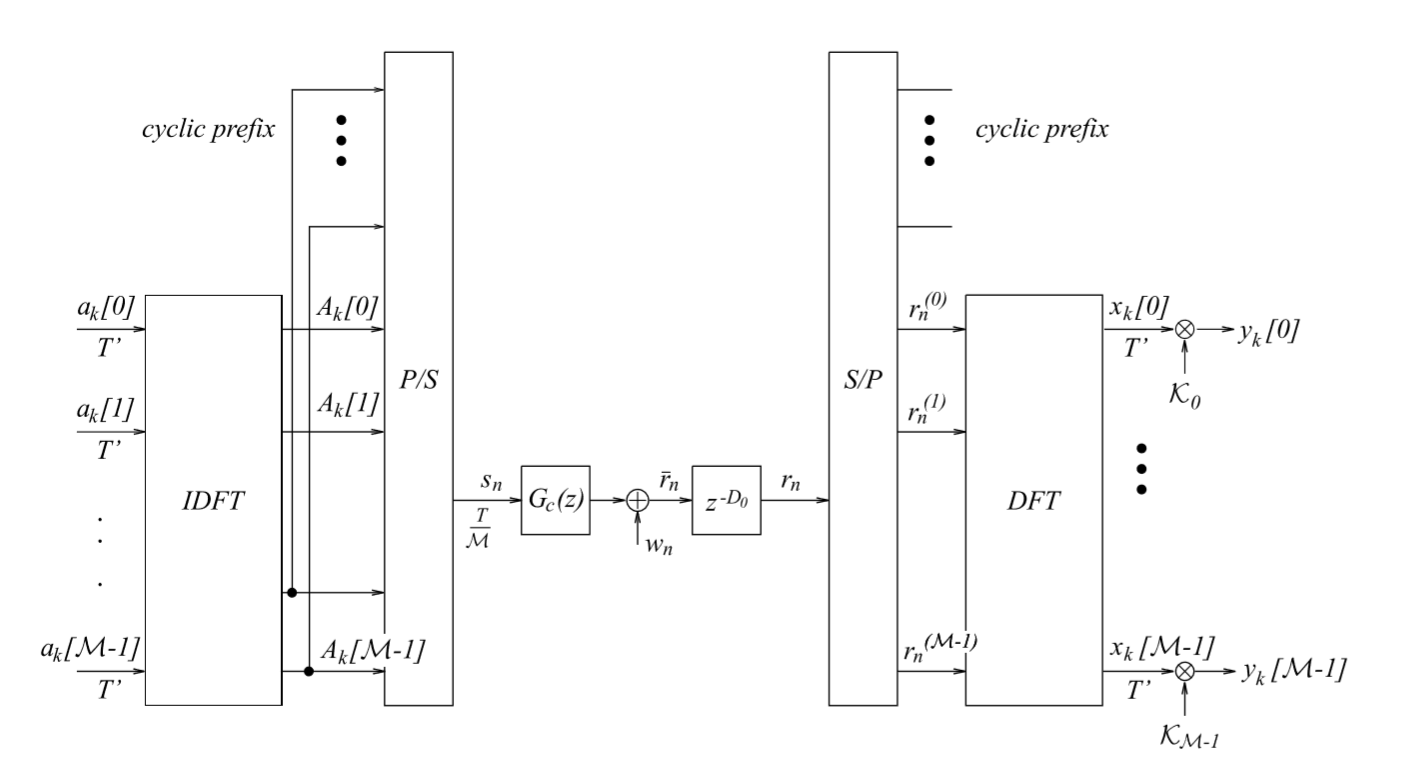
\includegraphics[width=14cm]{OFDM}
	\caption{Block diagram of a DMT system with cyclic prefix and frequency-domain equalizer.}\label{ofdm}
\end{figure}


We exploited the concept of circular convolution to obtain a convolution in the time domain as a product of finite length vectors in the frequency domain. To do so, we extended the block of samples $\mathbf{A}_k$ by repeating $N_{px}=18$ elements before transmitting through the channel. The value of $N_{px}$ was chosen equal to the support of the equivalent channel impulse response $h(mT_{OFDM})$. In particular, after the modulation, each block of samples is cyclically extended by copying the $N_{px}$ sample $A_k[\mathcal{M}-N_{px}],\dots,A_k[\mathcal{M}-1]$ in front of the block. After the P/S conversion, where the $N_{px}$ samples of the cyclic extension are the first to be sent, the $N_{px}+\mathcal{M}$ samples are transmitted over the channel.  At the receiver, blocks of samples of length $N_{px}+\mathcal{M}$ are taken; the boundaries between blocks are set such that the last $\mathcal{M}$ samples depend only on the elements of only one cyclically extended block of samples. The first $N_{px}$ samples of a block are thus discarded. \\
The resulting vector $\mathbf{r}_k$ can be expressed as 
\begin{equation}
\mathbf{r}_k = \mathbf{\Xi}_k\mathbf{g}_C + \mathbf{w}_k
\end{equation}
where 

\begin{itemize}
	\item $\mathbf{g}_C$ is the $\mathcal{M}$-component vector of the channel impulse response extended with $\mathcal{M}-N_{px}-1$ zeros;
	\item $\mathbf{\Xi}_k$ is an $\mathcal{M}$ $\times$ $\mathcal{M}$ circulant matrix, given by
	\begin{equation*}
	\mathbf{\Xi}_k = \begin{bmatrix}
						A_k[0] & A_k[\mathcal{M}-1] & \cdots & A_k[1] \\
						A_k[1] & A_k[0] & \cdots & A_k[2] \\
						\vdots & \vdots & \ddots & \vdots \\
						A_k[\mathcal{M}-1] & A_k[\mathcal{M}-2] & \cdots & A_k[0]
	\end{bmatrix}
	\end{equation*} \\
	
	\item $ \mathbf{w}_k$ is a vector of additive noise. 
\end{itemize}

Moreover, since $\mathbf{\Xi}$ is a circulant matrix, it satisfies the property

\begin{equation}\label{property}
\mathbf{F}_\mathcal{M} \mathbf{\Xi}_k \mathbf{F}_\mathcal{M}^{-1} = \text{diag}\{\mathbf{a}_k\}
\end{equation}

Defining the DFT of the vector $\mathbf{g}_C$ as $\mathbf{G}_C = \mathbf{F}_\mathcal{M}\mathbf{g}_C$ and using equation \eqref{property}, we can express the demodulator output as 

\begin{equation}
\mathbf{x}_k = \mathbf{F}_\mathcal{M}\mathbf{r}_k = \text{diag}\{\mathbf{a}_k\}\mathbf{G}_C + \mathbf{W}_k
\end{equation}

Finally, to equalize the channel using the zero-forcing criterion, $\mathbf{x}_k$ is multiplied by the diagonal matrix $\mathbf{K}$ which elements are simply given by

\begin{equation}
K_i = [\mathbf{F}]_{i,i} = \dfrac{1}{\mathcal{G}_{C,i}} \quad\quad\quad i=0,\dots \mathcal{M}-1
\end{equation}

Therefore the input to the data detector is given by

\begin{equation}\label{zfc}
\mathbf{y}_k = \mathbf{K}\mathbf{x}_k = \mathbf{a}_k+ \mathbf{K}\mathbf{W}_k
\end{equation}


\begin{figure}[H]
	\centering
	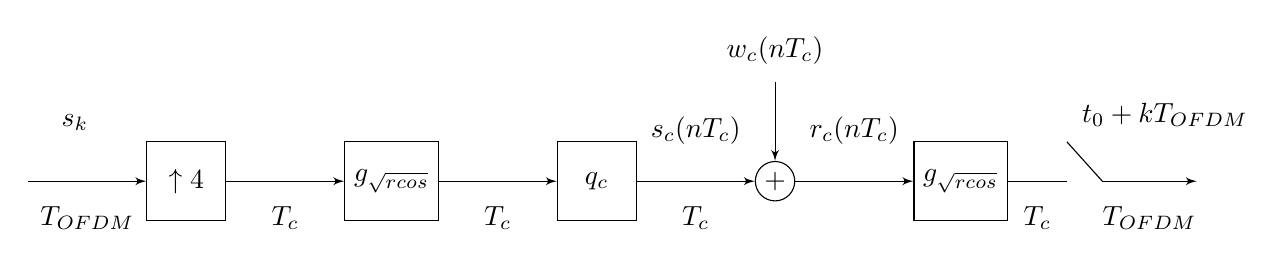
\begin{tikzpicture}[auto,>=latex']
	\tikzstyle{block} = [draw, rectangle, minimum height=1cm, minimum width=1cm]
	
	\node [coordinate, label={[label distance=0.6cm]60:$s_k$}] (start) {};
	\node [block, right = 1.5cm of start] (intpl){$\uparrow 4$};
	\node [coordinate, right = 0.75 cm of intpl] (c1) {};
	\node [block, right = 1.5cm of intpl] (imp){$g_{\sqrt{rcos}}$};
	\node [block, right = 1.5cm of imp] (qc){$q_c$};
	
	\node [draw, circle,minimum size=0.5cm,inner sep=0pt, right = 1.5cm of qc] (sum1){$+$};
	\node [coordinate, right = 0.75cm of imp] (c2) {};
	
	\node [coordinate, label={[label distance=0.1cm]90:$w_c(nT_c)$}, above = 1cm of sum1] (wgn) {};
	
	\node [block, right = 1.5cm of sum1] (matchedf){$g_{\sqrt{rcos}}$};
	\node [coordinate, right = 0.75 cm of matchedf] (c0) {};
	\node [coordinate, above = 0.5 cm of c0, label={[label distance=0.1cm]45:$t_0 + kT_{OFDM}$} ] (c1) {};

	\node [coordinate, right = 1.2cm of matchedf] (c2) {};

	\node [coordinate, right = 1.2cm of c2] (end) {};
	
	\draw [->] (start) --node[label={[label distance=0.2cm]270:$T_{OFDM}$}]{} (intpl);
	\draw [->] (intpl) --node[label={[label distance=0.2cm]270:$T_c$}]{} (imp);
	\draw [->] (imp) --node[label={[label distance=0.2cm]270:$T_c$}]{} (qc);
	\draw [->] (qc) --node[label={[label distance=0.2cm]270:$T_c$},  label={[label distance=0.1cm]90:$s_c(nT_c)$}]{} (sum1);
	\draw [->] (wgn) --node[]{} (sum1);
	\draw [->] (sum1) --node[label={[label distance=0.1cm]90:$r_c(nT_c)$}]{} (matchedf);
	\draw [-] (matchedf) --node[label={[label distance=0.2cm]270:$T_c$}]{} (c0);
	\draw [-] (c1) --node[]{} (c2);
	\draw [->] (c2) --node[label={[label distance=0.2cm]270:$T_{OFDM}$}]{} (end);

	
	\end{tikzpicture}
	\caption{Channel model for the OFDM transmission.}
	\label{Model_OFDM} 
\end{figure}

\clearpage
\subsection*{Detection}
At the detection point, we implemented the following system

\begin{figure}[H]
	\centering
	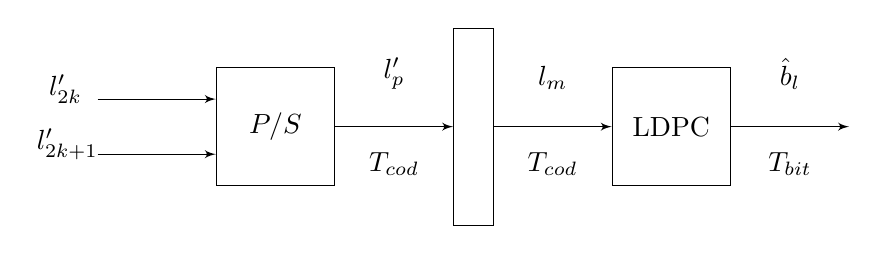
\begin{tikzpicture}[auto,>=latex']
	\tikzstyle{block} = [draw, rectangle, minimum height=1cm, minimum width=1cm]
	
	\node[draw, rectangle, minimum height=1.5cm, minimum width=1.5cm](llr) {$P/S$};
	
	\coordinate[above = 0.35cm of llr.west](a1){};
	\coordinate[left = 1.5cm of a1](llr1){};
	
	\coordinate[below = 0.35cm of llr.west](a2){};
	\coordinate[left = 1.5cm of a2](llr2){};
	
	\node [draw, rectangle, minimum height=2.5cm, minimum width=0.5cm, right = 1.5cm of llr] (deinterl) {};
	
	\node [draw, rectangle, minimum height=1.5cm, minimum width=1.5cm, right = 1.5cm of deinterl] (decoder) {LDPC};
	
	\coordinate[right = 1.5cm of decoder](end){};
	
	\draw [->] (llr1) --node[label={[label distance=0.7cm]180:$l'_{2k}$}]{} (a1);
	\draw [->] (llr2) --node[label={[label distance=0.5cm]180:$l'_{2k+1}$}]{} (a2);
	\draw [->] (llr) --node[label={[label distance=0.2cm]270:$T_{cod}$}, label={[label distance=0.1cm]90:$l'_p$}]{} (deinterl);
	\draw [->] (deinterl) --node[label={[label distance=0.2cm]270:$T_{cod}$}, label={[label distance=0.1cm]90:$l_m$}]{} (decoder);
	\draw [->] (decoder) --node[label={[label distance=0.2cm]270:$T_{bit}$}, label={[label distance=0.1cm]90:$\hat{b}_l$}]{} (end);
	
	\end{tikzpicture}
	\caption{Decoding scheme}
\end{figure}

For the single carrier transmission, the output of the DFE filter is a sequence of QPSK symbols $y_k$. These are decoded exploiting the LLR representation given by 

\begin{equation}\label{LLR}
l'_{2k} = -2\dfrac{\mathcal{R}[y_k]}{\sigma_i^2}
\end{equation}

\begin{equation}\label{LLR1}
l'_{2k+1} = -2\dfrac{\mathcal{I}[y_k]}{\sigma_i^2}
\end{equation}

where $\sigma_i^2 = \dfrac{J_{min}-\sigma_a^2 |1-\psi_D|^2}{|\psi_D|^2}$. \\ 
The generated data stream, which length is twice that of $y_k$, is \textit{deinterleaved} and decoded by the LDPC decoder provided. The final output $\hat{b}_l$ is compared with the initial data $b_l$ to count the number of errors introduced by the channel, and then $P_{bit}$ is finally computed as 

\begin{equation}\label{Pbit}
P_{bit} = \frac{\text{number of errors}}{\text{number of sent bits}}
\end{equation}

For the OFDM transmission $y_k$ is a matrix with $\mathcal{M}=512$ rows corresponding to the output of the $\mathcal{M}$ subchannels. Each LLR element is computed using equations \eqref{LLR} and \eqref{LLR1}, with the only difference that now $\sigma_i^2 = \frac{1}{2}\sigma_w^2 \cdot \mathcal{M} \cdot |K|^2 $. The final LLR vector is generated in such a way that two consecutive values at position \textit{i} and \textit{i+1} corresponds to the real and imaginary part of the same symbol in $y_k$. This operation is computed for all columns. The resulting vector is deinterleaved and decoded with the same procedure of the single carrier transmission. Finally the \textit{bit error probability} was computed using equation \eqref{Pbit}.

\clearpage
The filters we used are given as follow.

\begin{figure}[H]
	\centering
	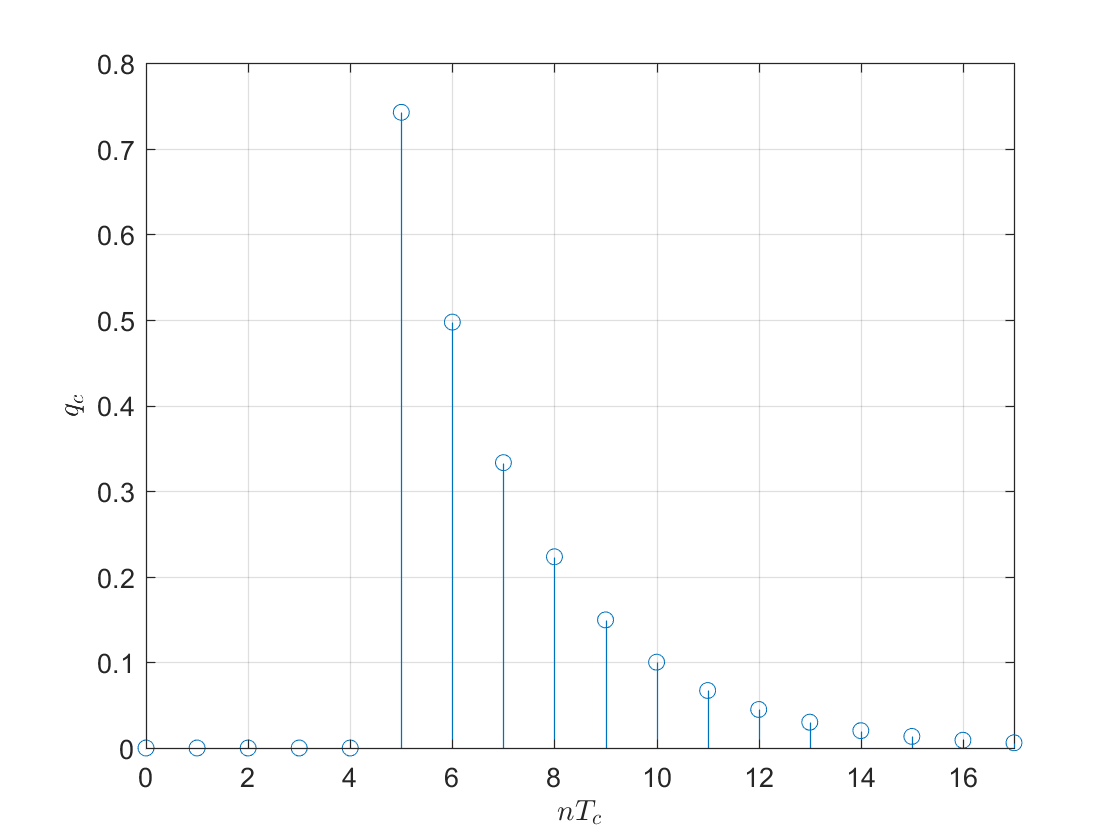
\includegraphics[width=14cm]{qc}
	\caption{Impulse response of the filter $q_c$.}
\end{figure}

\begin{figure}[H]
	\centering
	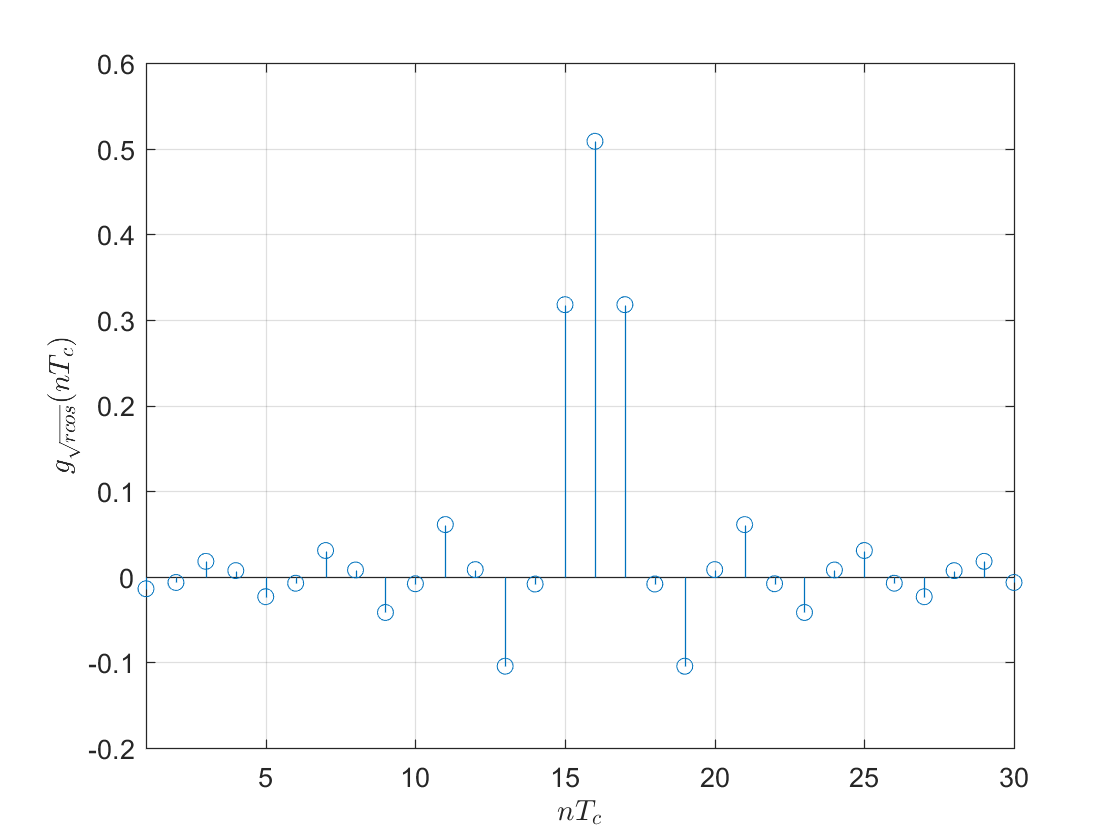
\includegraphics[width=14cm]{gsrrc_1}
	\caption{Impulse response of the square root raised-cosine filter.}
\end{figure}

\begin{figure}[H]
	\centering
	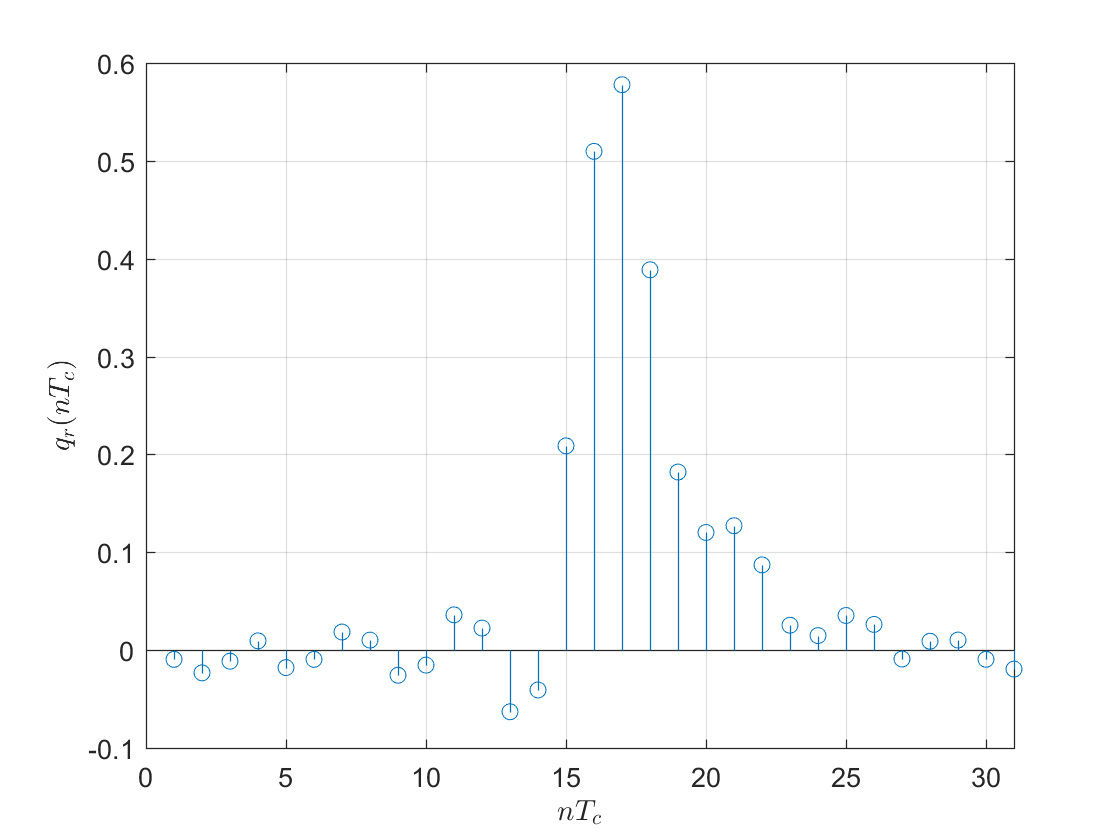
\includegraphics[width=14cm]{qr}
	\caption{Equivalent channel impulse response $q_r(nT_c) = g_{\sqrt{srrc}}(nT_c)*q_c(nT_c)*g_{\sqrt{srrc}}(nT_c)$.}\label{}
\end{figure}

\begin{figure}[H]
	\centering
	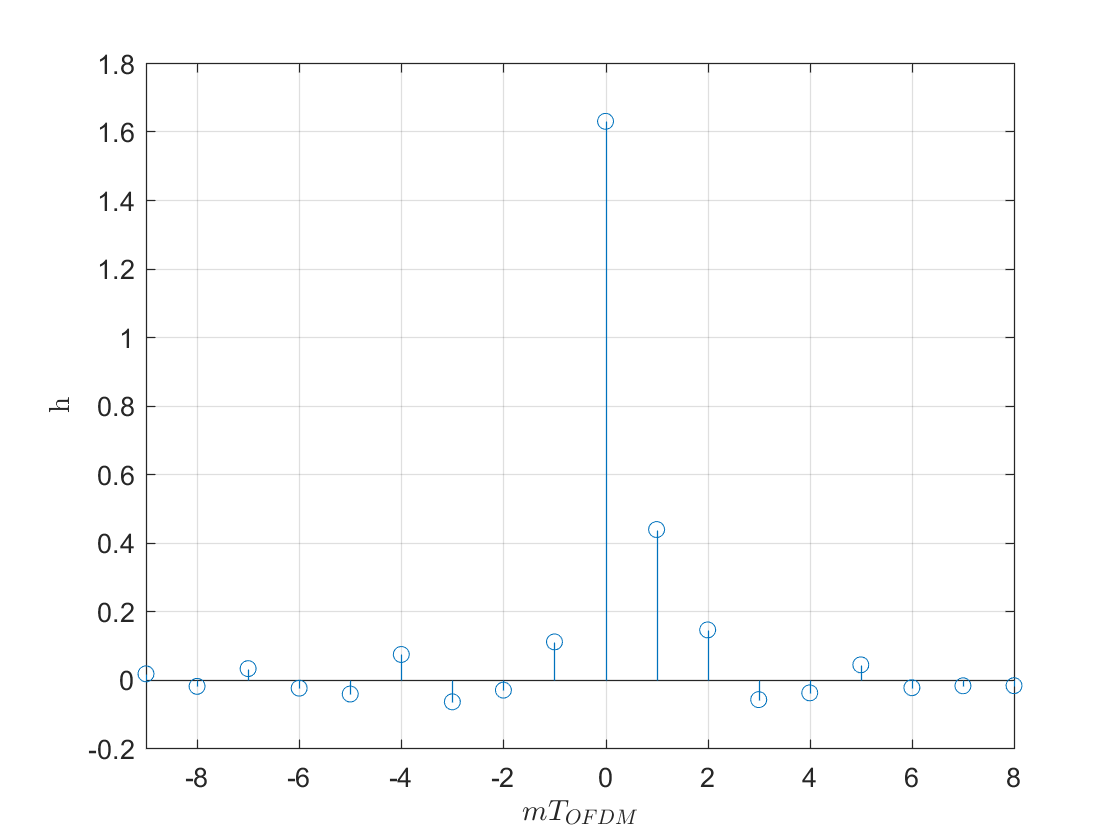
\includegraphics[width=14cm]{h}
	\caption{Equivalent channel impulse response after the downsampling, given by $h(mT_{OFDM}) = q_R(t_0+mT_{OFDM})$. Since $h$ has length 18, we chose $N_{px}=18$ as the \textit{prefix length}.}
\end{figure}

\begin{figure}[H]
	\centering
	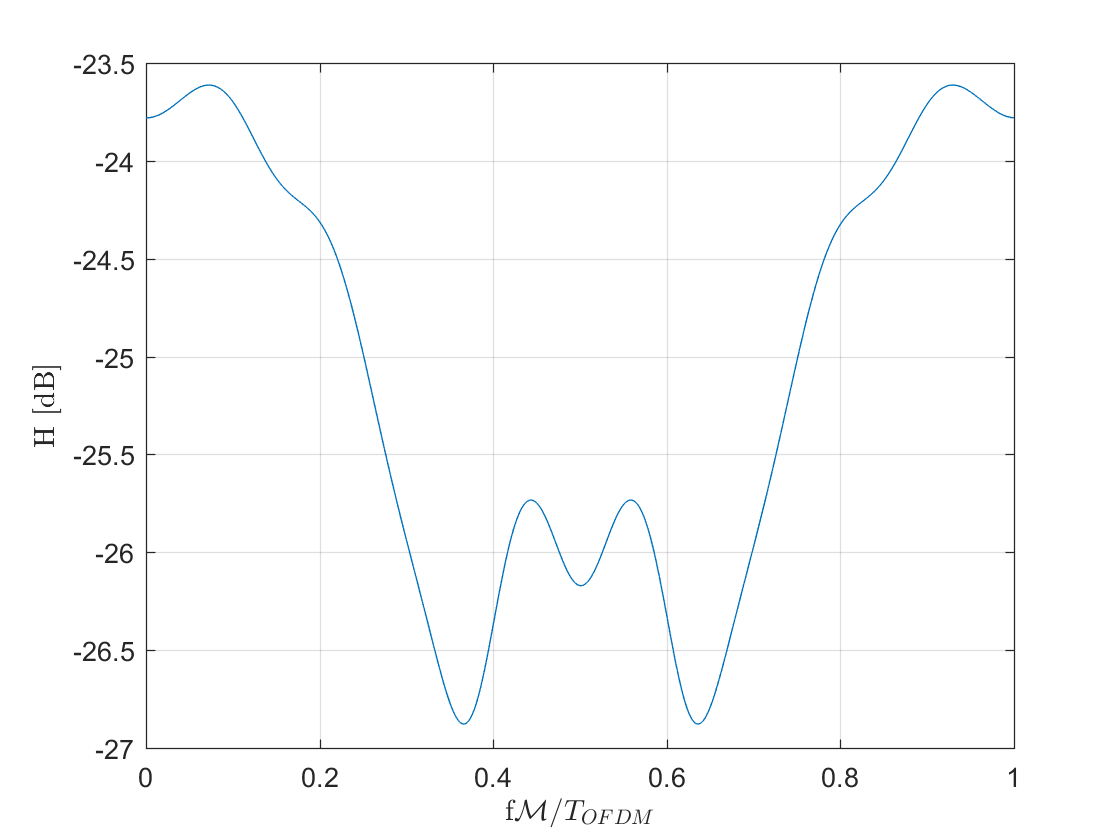
\includegraphics[width=14cm]{H_fft}
	\caption{FFT of the equivalent channel impulse response $h$ computed over $\mathcal{M}$ samples.}
\end{figure}

\begin{figure}[H]
	\centering
	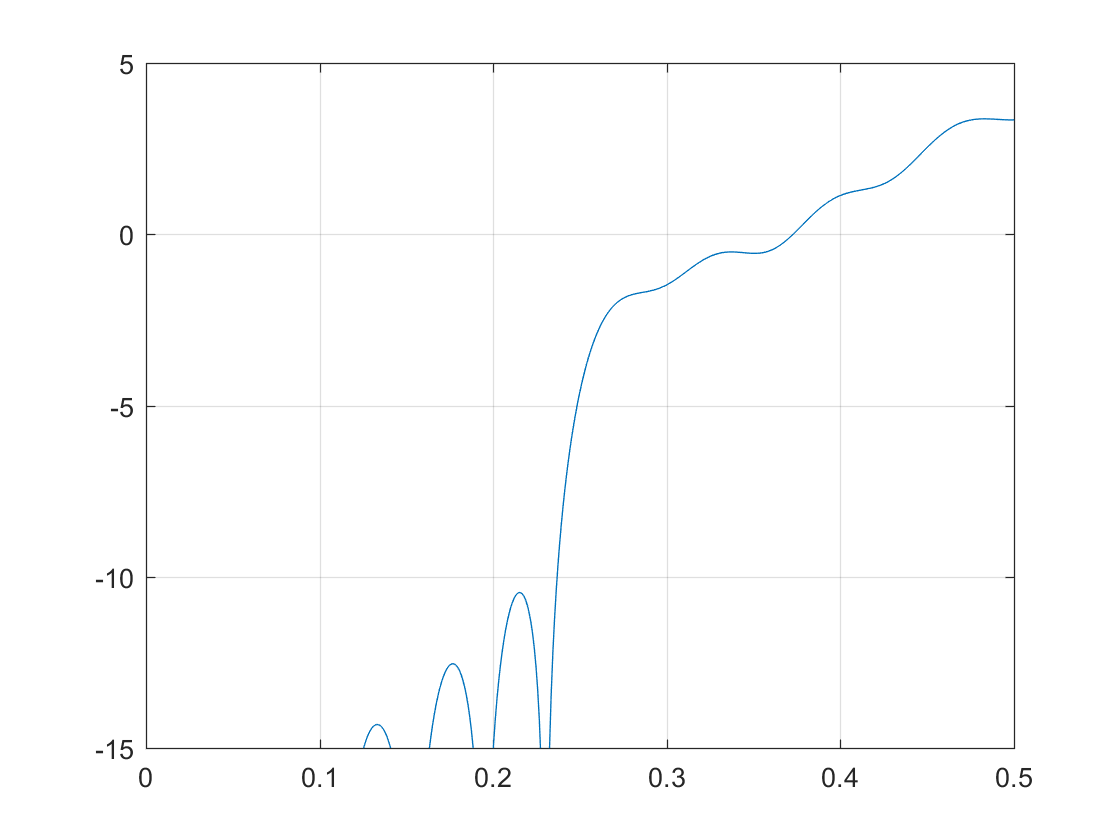
\includegraphics[width=14cm]{Q_r}
	\caption{Frequency response of the \textit{square root rised cosine} filter.}\label{}
\end{figure}

\begin{figure}[H]
	\centering
	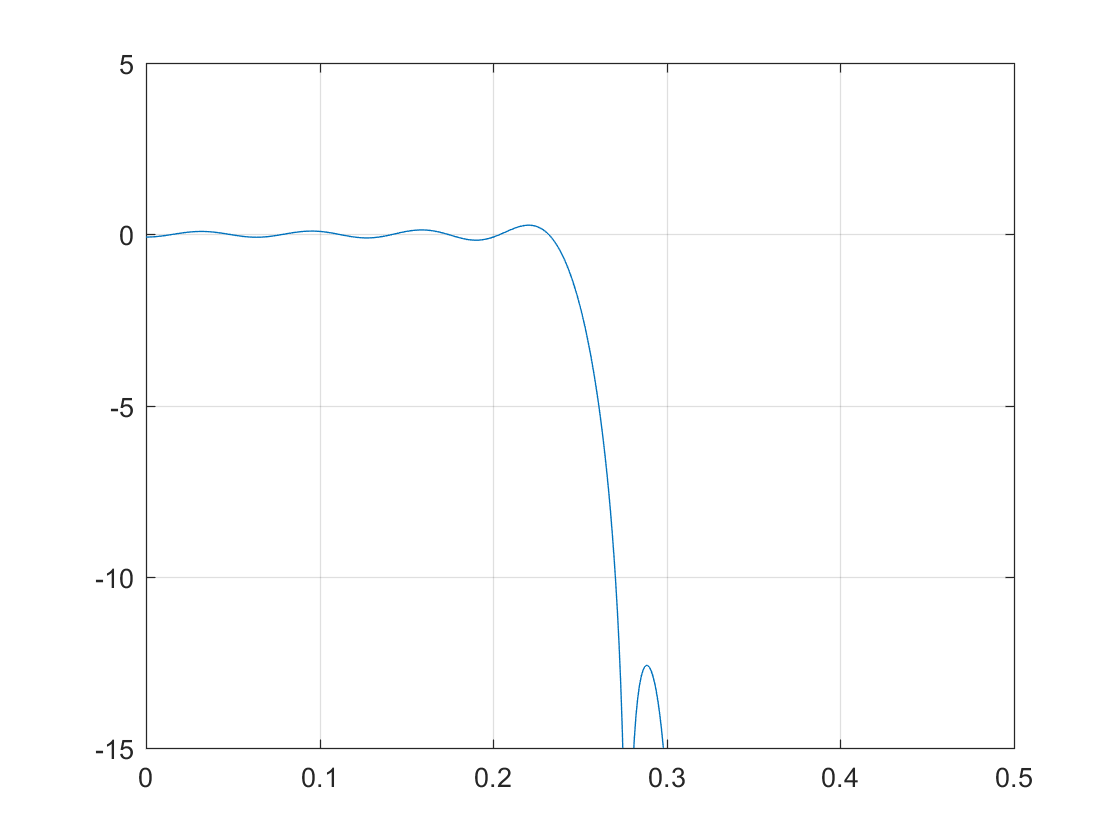
\includegraphics[width=14cm]{G_srrc}
	\caption{}\label{}
\end{figure}

\subsection*{Bit Error Probabilities}
Here the $P_{bit}$ obtained for the different configurations are given as function of the SNR $\Gamma$. \\
For the uncoded data transmission, the DFE receiver shows better performances. This is to be expected since the channel is well equalized by the \textit{decision feedback equalizer} filter; this can be noted by observing Figure [9] of homework 3, where the overall impulse response $\psi$ presents no precursors. On the other hand, the OFDM transmission system shows worse performances due to the fact that the zero-forcing criterion amplifies the noise signal components, as given in equation \eqref{zfc}. \\
For the coded data transmission, the DFE still shows good performances being only 1 dB over the AWGN bound. The OFDM system, however, thanks to the LDPC encoding scheme, performs even better.  

\begin{figure}[H]
	\centering
	\includegraphics[width=14cm]{uncoded}
	\caption{Simulated $P_{bit}$ for the uncoded transmission.}\label{uncoded}
\end{figure}

\begin{figure}[H]
	\centering
	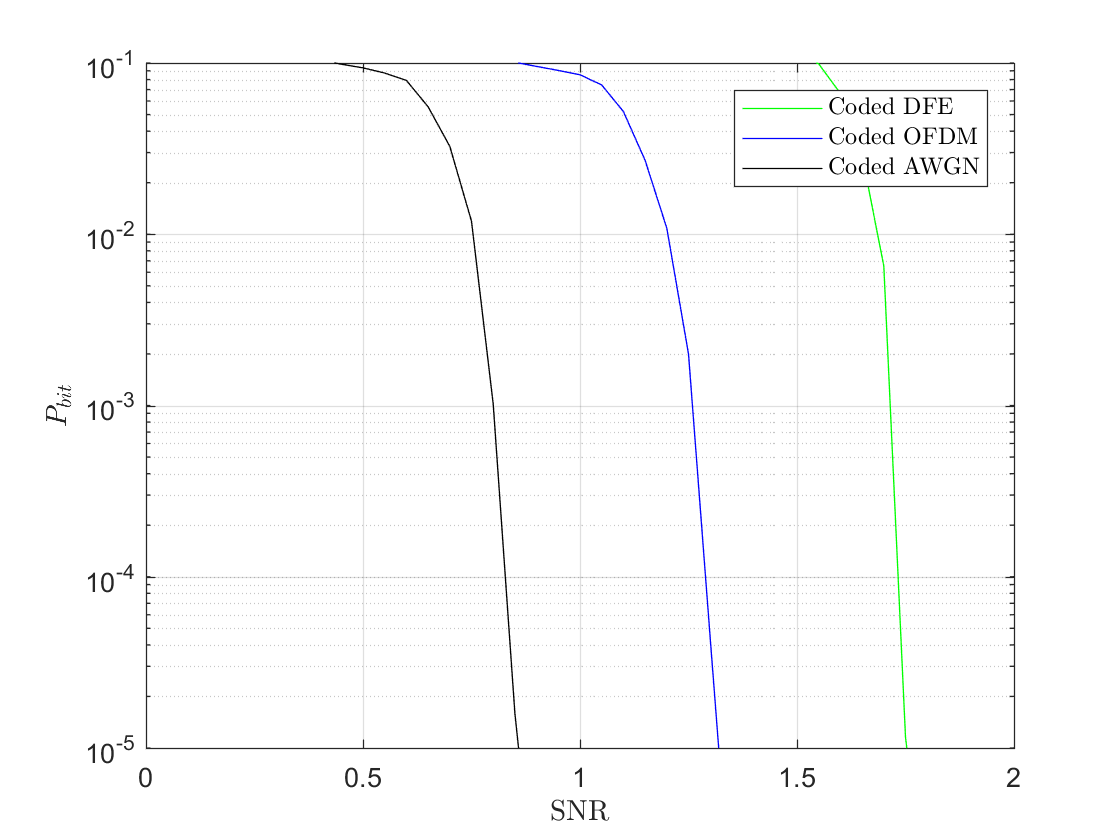
\includegraphics[width=14cm]{coded}
	\caption{Simulated $P_{bit}$ for the coded transmission.}\label{coded}
\end{figure}

\begin{thebibliography}{15}
	\bibitem{nevio<3}
	Nevio Benvenuto, Giovanni Cherubini,
	\textit{Algorithms for Communication Systems and their Applications}. 
	Wiley, 2002.
\end{thebibliography}

%\begin{figure}[H]
%	\centering
%	\begin{tikzpicture}[auto,>=latex']
%	\tikzstyle{block} = [draw, rectangle, minimum height=1cm, minimum width=1cm]
%	
%	\foreach \y in {0, 2, ..., 6}
%		{ \node [block] (0\y) at (0, \y) {$ \uparrow M$};}
%		
%	\foreach \y in {0, 2, ..., 6}
%	{ \node [block] (1\y) at (2, \y) {$z^{-\y} H(z)$};}
%	
%	\foreach \y in {0,2,...,6}  
%		\draw [->] (0\y)-- (1\y);
%		
%	\node [draw, circle,minimum size=0.5cm,inner sep=0pt] (sum) at (5,3) {$+$};
%		
%	\foreach \y in {0,2,...,6}  
%	\draw [->] (1\y)-- (sum);
%	
%	\end{tikzpicture}
%\end{figure}

\end{document}